% ------------------------------------------------------------
% Page 94 bis
% ------------------------------------------------------------

\begin{tikzpicture}[remember picture,overlay]
    \node[
        anchor=south west,
        inner sep=0pt,
        opacity=0.60
    ] at (current page.south west) {%
        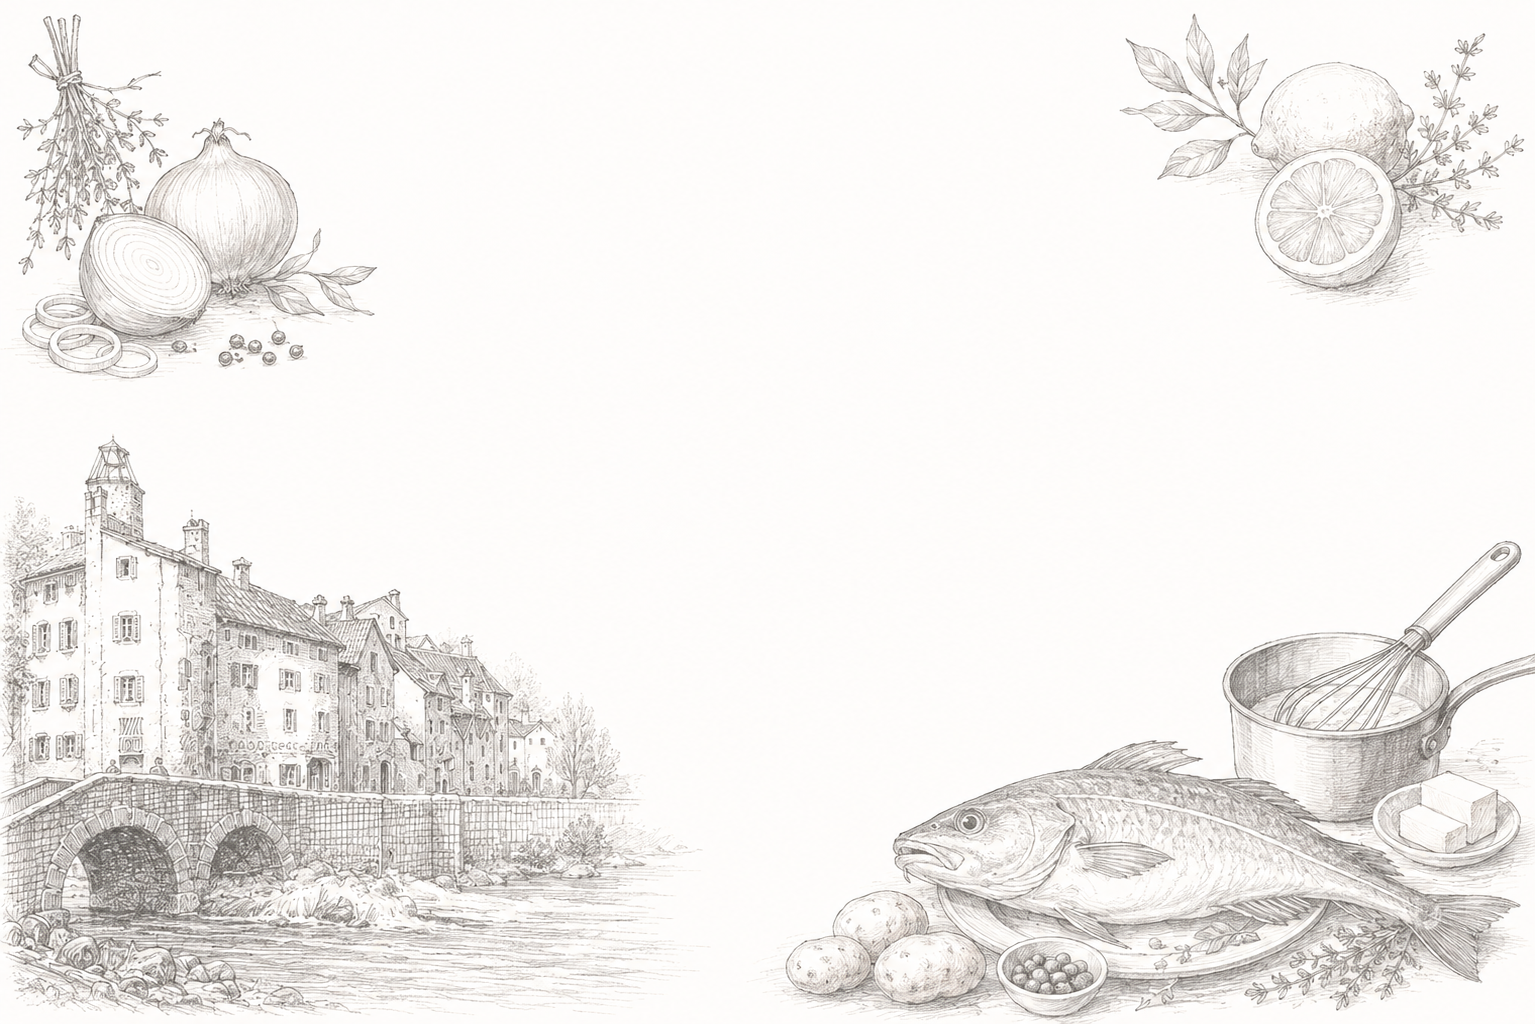
\includegraphics[
            width=\paperwidth,
            height=\paperheight
        ]{imgs/101}%
    };
\end{tikzpicture}

\sectiondate{Recette de la Morue à la Sauce Blanche}{}

{\fontspec{Comic Sans MS}
\large

\vspace{25mm}

Faire dessaler la morue, un ou deux jours à l’eau froide en renouvelant l’eau
régulièrement.

La mettre à cuire dans de l’eau froide avec des rondelles de citrons, des
tranches d’oignons, thym, laurier, poivre et un morceau de beurre.\\

Quand la morue est cuite la retirer et la tenir au chaud, faire cuire les pommes
de terre avec la même eau sans les éplucher auparavant.\\

Dresser le poisson sur un plat, les pommes de terre épluchées une fois cuites,
autour.\\

\textbf{Servir avec une sauce blanche}

Mettre dans une casserole 30 g de beurre frais, laisser fondre à blanc, ajouter
deux cuillerées de farine fine ; faire cuire quelques minutes à feu doux, en
remuant avec un fouet sans laisser prendre couleur. Y verser doucement de
l’eau bouillante, toujours en remuant avec le fouet pour éviter les grumeaux.\\

Saler, poivrer, laisser faire un bouillon et y incorporer, par petits morceaux,
30 nouveaux gr. de beurre ou un pot de crème.\\

Ne plus laisser cuire pour conserver à la crème son goût de beurre frais.

Si on en trouve à l’épicerie du coin, ajouter des câpres avant de servir.

Terminer par une liaison à l’œuf et un filet de jus de citron.}

\begin{center}
Quel délice ! Bon appétit !
\end{center}

\begin{flushright}
Marianne Loupiac\\
Juin 2006
\end{flushright}
